\documentclass[11pt,paper=letter]{scrartcl}
\usepackage[alttitle]{cjquines}

\begin{document}

\title{Graph theory}
\author{Carl Joshua Quines}
\date{June 7, 2019}

\maketitle

\subsubsection*{Definitions}

Graph, vertices, edges, adjacent, incident, simple graph. Subgraph, induced subgraph, spanning subgraph. Isomorphic graphs. Neighbor, degree, minimal degree $\delta$, maximal degree $\Delta$. Path $P_n$, length, cycle $C_n$, complete graph $K_n$. Connected, disconnected, connected component. Tree, forest. Directed graph, indegree, outdegree.

All of these are on Wikipedia: just search for something like \href{https://www.google.com/search?q=tree+graph+theory}{tree graph theory} on Google.

\subsubsection*{Some lemmas}

\begin{enumerate}
  % edge counting
  \item (Handshake) The sum of the degrees is twice the number of edges. Thus, the number of vertices with an odd degree is even.

  \textbf{Sketch:} Each edge contributes $2$ to the sum of the degrees.
  % induction
  \item (Veblen) The edges can be partitioned into cycles if and only if each vertex has even degree.

  \textbf{Sketch:} If the edges can be partitioned into cycles, it's easy to show each vertex has even degree. For the other direction, first prove that a cycle exists. Then remove it from the graph and induct.

  \textbf{Remark:} The proper way to think about induction in graph theory is usually ``breaking down'' rather than ``building up''. An induction proof in graph theory usually looks like this:
  \begin{enumerate}
    \item Suppose that the theorem is true for $n-1$.
    \item Take a graph with $n$. Remove something so that it has $n-1$. Use the inductive hypothesis to get the theorem for $n-1$.
    \item Add the something you removed back to get $n$. Show that it still works, or that the theorem is true for $n$.
  \end{enumerate}
  That is, rather than just ``add something to $n-1$'', it looks more like ``remove something from $n$ to get $n-1$, then add it back to get $n$.'' That way, you're guaranteed to cover \emph{all} possibilities.

  % assume the existence of a maximum object
  \item A graph has a cycle of length $\geq \delta + 1$. A graph has a path of length $\geq \delta$.

  \textbf{Sketch:} Take a longest path. Let $v$ be its last endpoint. Every one of $v$'s neighbors lie on the path, otherwise we can make the path longer. So the path has at least $\text{deg}\,v + 1$ vertices: the $\text{deg}\,v$ neighbors of $v$ and $v$ itself. The task of finding the cycle is left to the reader.

  \item A graph can be partitioned into two sets $V_1$ and $V_2$ such that any vertex in $V_1$ has at least as many neighbors in $V_2$ as in $V_1$ and vice versa. %take the max cut

  \textbf{Sketch:} Take the partition with the most edges between $V_1$ and $V_2$. Suppose that $v \in V_1$ does not satisfy the condition. Then move $v$ to $V_2$ and show that it satisfies now. The process increases the number of edges between $V_1$ and $V_2$, contradiction. 
\end{enumerate}

\subsubsection*{Trees}

A tree is a connected graph with no cycles. All of these can be cited without proof:

\begin{enumerate}
  \item A tree is a connected graph with the minimum number of edges. (= We can't remove an edge from the tree without making it disconnected.)
  \item A tree is a connected graph with $n$ vertices and $n-1$ edges.
  \item A tree has at least two vertices of degree one.
  \item A tree has a unique path between any two vertices.
  \item A tree has no cycles and has the maximum number of edges. (= We can't add an edge to the tree without making a cycle.)
  \item Any connected graph has a spanning subgraph that is a tree (called a \emph{spanning tree}).
\end{enumerate}

\subsubsection*{Problems}

Not in order; sorry!

\begin{enumerate}
  \item (Putnam 1957) Let $S$ be a set of points in the plane such that the greatest distance between two points of $S$ is $1$. Show that at most $n$ pairs of points in $S$ are at distance $1$ apart.

  \textbf{Sketch:} Induction. If every vertex has degree $\le 2$, we are done (why?). If a vertex has degree $\ge 3$, it has a neighbor of degree $1$ (why?). So remove the vertex of degree $1$ and induct.

  \item (MOSC 2016) In a party attended by $2015$ guests, among any $5$ guests at most $6$ handshakes have been exchanged. Determine the maximum total number of handshakes.

  \textbf{Sketch:} Induction. Replace $2015$ with $k$. If $k = 2n$, then the answer is $n^2$; if $k = 2n - 1$, then the answer is $n(n-1)$. To prove that this is attainable, use the construction shown earlier. To prove that it can't be greater than the answer, we use induction. Base case is $k = 5$. We'll only do the case $2n - 1 \implies 2n$; the reader should fill in the details of the other case. 

  Suppose that a graph with $2n$ vertices has $\ge n^2 + 1$ edges and it satisfies the condition in the problem. By pigeonhole, there exists a vertex with degree $\le n$. (Why? Use handshake.)

  By removing this vertex, the remaining graph has $2n-1$ vertices and $\ge n^2 - n + 1$ edges, but it also satisfies the condition. (Why?) But this contradicts the inductive hypothesis! So the graph must have $\le n^2$ edges.

  \textbf{Remark:} A solution template for any problem that asks for the maximum of $X$ is this:
  \begin{enumerate}
    \item ``We claim that the maximum of $X$ is $M$.''
    \item ``We prove that $M$ is attainable,'' and give a construction that $M$ is possible, or prove that $M$ can be attained. Even if this is trivial, you \emph{still} need to explain it.
    \item ``We prove that $X$ cannot be larger than $M$,'' and then given a proof why $X$ cannot be larger than $M$. 
  \end{enumerate}
  If this is your first time hearing this, read \href{http://web.evanchen.cc/handouts/english/english.pdf}{Evan Chen's Remarks on English}. It is not long.

  \textbf{Remark:} Try Japan 1998: A country has $1998$ airports connected by some direct flights. For any three airports, some two are not connected by a direct flight. What is the maximum number of direct flights that can be offered? Answer: $999^2$.

  \item The complete graph is the union of paths of distinct lengths.

  \textbf{Hint:} Stare at the following picture:
  \begin{center}
    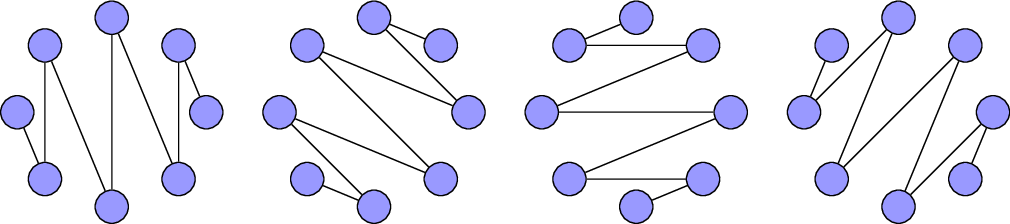
\includegraphics[width=6in]{1.png}
  \end{center}

  (Picture stolen from \href{https://math.stackexchange.com/questions/2130583/partition-edges-of-complete-graph-into-paths-of-distinct-length}{Rebecca J. Stone's answer on math.SE}.)

  \item A graph with $\delta \geq k$ has a subgraph isomorphic to any given tree with $k+1$ vertices.

  \textbf{Sketch:} Induction. Take out a vertex from the tree with degree one (why does it exist?), to get a tree with $k$ vertices. By hypothesis, it's a subgraph. Now add the vertex back in (why can we always do this?)

  \textbf{Remark:} Try ELMO Shortlist 2011: Let $T$ be a tree with $t$ vertices, and $G$ be a graph with $n$ vertices. Show that if $G$ has $\geq (t-1)n$ edges, then it has a subgraph isomorphic to $T$.

  \item (Dirac) A graph with $n$ vertices and $\delta \geq n/2$ has a cycle that passes through all the vertices.

  \textbf{Sketch:} Essentially the same idea as Lemma 3 from earlier: we consider the longest path and show it works.

  Consider the longest path with vertices $v_1, v_2, \ldots, v_t$. All the neighbors of $v_1$ and $v_t$ lie on the path. (Why?) In particular, this means that there is some $v_k$ and $v_{k+1}$ such that $v_1$ is adjacent to $v_k$ and $v_t$ is adjacent to $v_{k+1}$. (Why? Use the degree condition.) So we can complete this to form a cycle of length $t$.

  Suppose that the cycle of length $t$ does not include all $n$ vertices. Then it's missing some vertex, say, $v$. Then you can connect $v$ to the cycle to make a longer path than $v_1, v_2, \ldots, v_t$ (why?), contradiction.

  \item (ELMOSL 2011) The indegree and outdegree of each vertex in a directed graph is $2$. Show that we can partition the graph into three sets such that no vertex is in the same set as both the vertices it points to.

  \textbf{Sketch:} Essentially the same idea as Lemma 4 from earlier: consider the partition with most cross edges and show that it works.

  Take the partition with the most edges in between the sets. Suppose that a vertex $v$ does not satisfy the condition. Show that it is possible to move $v$ to some other set, such that the number of edges between the sets increases, and that $v$ satisfies the condition. This is a contradiction.
\end{enumerate}

\subsubsection*{Bonus}

\begin{enumerate}
  \item In $K_n$, we change each edge to an arrow. This is called a \emph{tournament}. Show that there is a path following the arrows that passes through all the vertices. (Hint: Induct on $n$.)

  \item (Romania 2006) The edges of a polyhedron are oriented such that every vertex has at least one edge directed toward it, and at least one edge directed away from it. Show that some face of the polyhedron has its edges oriented in a circle.

  \item (ISL 2004) Let $n \ge 4$ be an integer. We do the following graph operation: choose any $C_4$ subgraph, and remove any edge. Find the least number of edges of that can be obtained by repeated applications of this operation on $K_n$.
\end{enumerate}

\subsubsection*{Read more?}

Reinhard Diestel's \emph{Graph Theory} is a good book with an electronic edition that is \href{http://www.esi2.us.es/~mbilbao/pdffiles/DiestelGT.pdf}{\textbf{free} on the author's website}. 

References used in preparing this problem set are Bollob\'as's Modern Graph Theory and Sriram's \href{https://artofproblemsolving.com/community/c6h601134}{Olympiad Combinatorics}.

% \subsubsection*{Counting edges}

% % edge counting
% \begin{enumerate}
%   \item  % HANDSHAKE LEMMA
%   \item (Hungary 2010) There were $n$ people at a party. Sometimes $3$ persons played a game of cards. At the end of the party, it turned out that any three persons played in at most one game together and any two persons played exactly twice together. For which $n$ is this possible if $3 < n < 9$?
%   \item  %Mantel's
% \end{enumerate}

% \subsubsection*{Induction}

% % induction
% \begin{enumerate}
%   \item 
%   % \item A graph with average degree $d$ has a subgraph with minimum degree at least $d/2$.
%   \item 
%   \item (Romania 2006) The edges of a polyhedron are oriented such that every vertex has at least one edge directed toward it, and at least one edge directed away from it. Show that some face of the polyhedron has its edges oriented in a circle.
% \end{enumerate}

% \subsubsection*{Assume the existence of an extremal object}

% \begin{enumerate}
%   \item (Russia 2001) A company with $2n+1$ people has the following property: For each group of $n$ people, there exists a person amongst the remaining $n+1$ people who knows everyone in this group. Show that there exist a person who knows all the people in the company. %FTSOC no. Compliment of friendship graph has a dominating set with at least n vertices, contradicting the problem statement. 
% \end{enumerate}

\end{document}
